\chapter{Results: From Specification to End Product}
\label{ch:game}
\containsfigures{Results: From Specification to End Product}
\containslistings{Results: From Specification to End Product}
\containstables{Results: From Specification to End Product}

\chapterepigraph{Finishing races is important, but racing is more important.}{Dale Earnhardt}

% introduction for this chapter, is not a section



introduction
------------
Our project, irrelevent to implementation language has a very simliar foundation to all games, requiring networking between computers playing the game, graphics engine that can draw the game, assets/sprites for in game entities.

The game's implementation will be designed with an infrastructure that is at the core. All game features will run on top of this infrastructure, having little dependency on other game features, but having complete dependency on the infastrcture. This architecture allows very module design with regards to game features, allowing new game features to be added to the implementation only a slight modification of the infrastructure to include the new feature. By designing the architecture like this, It faciliates a release based schedule.

A high level specification is now available that specifices the elemnts of the game. To bring this high level specification to reality, the game design will be broken down into 3 major releases: Alpha, Beta 1, and Beta 2. Each release specifies the game features that must be in the game. Essentially the game design is broken down into game features, with higher priority game features being specified in earlier releases.
Alpha Release is primarily focused on building the game's Infrastructure, this is the core of the game with all the back end logic that is never seen by the player. By the end of Alpha 1 the game infrastructure is mostly complete, and the game is in a state where game logic can now be added on like modules with little dependency 
Beta 1 and Beta 2 are both game feature oriented, building on top of the existing infrastructure, adding features described in the specification. These releases will heavily focus on meeting the specification's specified game features.

Laying The Foundation
---------------------
Terminology was the first step in the conversion process from specification to working game. 
An initial ambiguity was that many of haskell libraries being looked into had a concept of 'world' which varied dramatically, which in term caused every member of the team to have a different meaning for the word. This caused many misunderstandings until an internal terminaology was devised within the team to describe common terms such as 'client state'. Once the terminology hurdle was solved, The team was able to share design ideas efficiently.

By the end of alpha Stage a working 'game' was needed, somethat that could be used as a base to start adding game features.

The infrastructure must provide a platform that the game features can be implemented ontop of, Hence it must contain:
\begin{itemize}
\item Server-Client communication
\item Rendering capabilities for assets
\item Game loop
\item Model of game components
\end{itemize}

Mistakes at this stage will cost heavily later down the line, because so much will dependend on the infrastructure. 

\begin{comment}

alpha stage layout
------------------
features wanted at this stage:
    - networking
    - server client loop
    - game update model (lock-step no no no)
    - ship move orders
    - world rendering(easy debugging)
    - more focus around infrastructure than features
    
    
  - lack of libraries, implemeintg our own networking, GUI library.
  - implementation of network library.
  - server and client not distinquished just yet
  - game loop
  - lock-step big part
    - arguments for and against
  - integration of assets into game
  - API for game how entities are added
  - how generating diffs will work

  - infrastructure components
    - networking
    - gameploop
    - how the server and client synchronize
    - graphics


\end{comment}


% sections

\section{Server-Client Sychronization}

\begin{comment}

this section talks about the decision for server client architecture.
server-client allows master copy to exist on server.

- master copy of world on server
- clients perform no logic, only apply updates to

we need to work out how the computers talked to each other very early on
2 considerations: peer 2 peer, client-server
  - advantages of peer 2 peer
  - advantages of peer server-client
  - why server-client chosen 
  - issues experienced with server-client
    - jumpy ship movements

\end{comment}

The game was designed around being multiplayer, so our first goal was to decide how they would talk to each other.
Since their was an arbitrary number of players (greater than 1), We needed a system that would scale, but would also be robust.
The game was expecting all players to be on the same LAN (Local Area Network), hence a high bandwidth was available for the communications.


% lockstep
%   - each client has the master copy of the world
%   - when a client does something, it tells all others
%   - problems:
%     - desycnhronization
%     - currupted client fucks up everyone

% simple server client
%   - it's what we've implemented
%   - no simulation on clients
%   - 1 server that has master copy
%   - server does all processing and sends updates to clients
%   - clients just render the world and send commands to server

% server client with simulation
%   - similar to simple server client but client does 'some' simulation. They in no way can effect the world.
%   - for instance if client knows ships destination and current location it can render the ship graciously moving instead of jumping on every update.


\section{Rendering the Game}

% old assets
% ----------
% ships made to look very big
% many prototypes
% merging assets with code, dynamic color

% master copy of assets in dropbox under 4y project/laith/design

One very important aspect of the client program is rendering the current game state to a display for the user to interact with. Creating a picture of the game to display requires a number of graphical assets to visually represent the various entities and scenery that make up the game world. For Project Serenity all of these graphics were created from scratch using Photoshop and Illustrator. Figure~\ref{fig:assets} shows a selection of some of the assets that were created for different entities.

% TODO INSERT FIGURE OF PLANETS AND SHIPS
% full page on planets, full ships

% TODO Chat about the actual rendering process. Thoughts:
%
% * World coordinates: all entities are located in world coordinates and a view of the world is drawn in this way first
% * Viewport: the display is scaled and translated by the current settings stored by the client
% * Along with the actual world there is some extra GUI that helps the player understand the current state of the game:
%      - Minimap
%      - Currently selected entity

The client uses these assets to draw the sector and place each player's ships in the correct locations. This is done by placing the assets using world coordinates in the 2D space defined by the dimensions of the sector. The picture that has been built up so far is then translated and scaled according to the current panning and zoom settings stored in the client. This allows the user to smoothly zoom in and out as well as scroll around the sector. There are optimisations that could have been performed, such as working out which entities would be displayed and only drawing them instead of drawing them and scaling them out of view, but in the end there were not required.

Along with the actual world there is some extra GUI elements to help the player keep track of the current state of the game. Firstly there is a minimap in the bottom left corner. This displays a schematic representation of the sector with the locations of friendly ships. The minimap allows the user to quickly check on the current status of their fleet. It was originally hoped that the minimap could be used to show extra events such as known locations of enemies and current attacks. It could also be enhanced by allowing the user's view to be transported to the location clicked on the minimap. However, core features were prioritised over this extra functionality, and so they are not implemented yet.

Figures~\ref{fig:gameplay} and \ref{fig:gameplay2} show how similar the resulting game was to the initial mockup made during the specification stage (see Figure~\ref{fig:mockup1}).

\begin{figure*}[p]
	\includegraphics[width=16cm]{res/serenityscreens/09-ingame1}
	\caption[][1em]{Screenshot during gameplay showing a planet, spacelanes, selected ships, and minimap.}
	\label{fig:gameplay}
\end{figure*}

\begin{figure*}[p]
	\includegraphics[width=16cm]{res/serenityscreens/10-ingame2}
	\caption[][1em]{Screenshot during gameplay showing a selected planet, spacelanes, a ship, and minimap.}
	\label{fig:gameplay2}
\end{figure*}

The second piece of GUI is the ship and planet selection indicators. When a user left clicks on an entity, or drags a selection box over a group of entities, they are selected and a dashed selection circle surrounds the entity. To make this feature easier to use a group selection does not select all entities within the drag area. Instead some are prioritised over others: ships are ranked above planets, and friendly ships are ranked above enemies. For example, if a selection is made over the entire sector then only the friendly ships will be selected. If a single entity is selected then details about it will be shown in the top left of the screen.

% TODO Talk about parallax because it's interesting? (Innovative?)

Another interesting piece of the rendering puzzle was to choose a colour as a unique visual representation for each player. This would be used to help players differentiate their ships from the enemy and to identify the planets that they own. A clever algorithm was used that would take a numerical player identifier and return a unique colour:\cite{ankerl2009}

\begin{equation*}
	colour(i) = HSV(i \times \phi^{-1} \mod 1, 1.0, 0.8)
\end{equation*}
\noindent
This function uses the HSV colour space using a fixed saturation and value, but modifying the hue to create equally bright and vibrant colours. The player's identifier, $i$, is used to step into the possible values for hue by multiplying it by the reciprocal of the golden ratio, $\phi$, modulo one. Due to the equidistribution theorem\sidenote{The equidistribution theorem states that the sequence $a, 2a, 3a, \ldots \mod 1$ is uniformly distributed when $a$ is an irrational number} this creates a sequence of colours that are evenly spread across the colour space. Using this method to generate team colours created visually pleasing colours that are suitably distinct from each other to be used for recognition.

\section{GUI}
<please insert shizzle here>
\section{Resources: The Currency of the Game}
\label{sec:resources}

The game was designed to include a resource system. Players would collect resources to be used to power their fleets. In this way, resources represent the currency of the game and a player's access to sufficient resources has a dramatic affect on their chances of winning a battle. There are three different types of resource: fuel, metal, and anti-matter. Each resource has a unique purpose in the game, requiring the player to modify their strategy according to the quantity of resources they have access to.

\begin{description}
\item[Fuel] Fuel is used to regenerate a ship's shields. As discussed previously, shields are vitally important to the protection of a ship since they prevent or reduce the amount of damage that is done to the ship's hull. Without fuel a ship would be much more vulnerable to attack since it is unable to replenish its shields. An extension to this concept would be to require ships to have fuel to power their shields at all, however, this potential dynamic has not been explored fully.

\item[Metal] If a ship's hull has been damaged then the supply of metal can be used to slowly repair it. Access to a greater quantity of metal allows a player to adopt a bolder strategy since their damaged ships can be brought back to full health if they are not destroyed completely. Without metal any damaged ships become easy prey for the enemy since they are unable to recover from attacks and will quickly be destroyed.

\item[Anti-matter] There are certain very powerful weapons that a ship can be equipped with. However, these weapons require a supply of anti-matter, the rarest of the three resources, to be used. Having access to anti-matter allows a player to unleash devastating attacks from these special weapons and could possibly turn the tide of battle in their favour.
\end{description}
\noindent
A player is able to mine resources from the planets that are under their control.\sidenote{See Section~\ref{sec:planetary-capture} on how to gain control of planets} As discussed in Section~\ref{sec:model}, each planet in the sector has a supply of resources that varies depending on its ecotype. Planets that are owned by a player will provide a constant trickle of resources to the player.

Although the framework for the resource system is in place, the actual usage of resources has not been implemented yet. This is because discussions about the mechanics of resource consumption never really came to a concrete conclusion. So, it was decided that it would be better to focus on the other planned features and to return to resources if there was time. The remainder of this section discusses the two potential resource systems that were debated.

% Two possible mechanics?
% 1. Ships have individual supplies that is drawn from the global supply if stationed at a friendly planet
% 2. Ships drain a global supply

The first possibility is that each ship in a player's fleet has an individual supply of resources. When the ship is stationed near to a friendly planet then it will be able to resupply from the player's global stockpile. The quantity of resources that an individual ship can store for use would be dependent upon its type, larger ships being able to carry more supplies than smaller ones. Once a ship leaves the safety of home territory and starts receiving damage or using special weapons it will start to drain its internal resource cache. The ship's supplies will eventually empty out and it would have to return to a home planet to receive any more. If a ship continues to battle without resources then it will eventually sustain damage that it is unable to repair and will be more likely to get destroyed.

The other option would be to only have a single global supply of resources. Ships would then drain that global stockpile as needed no matter where they are located in the sector. This mechanism would probably encourage more aggressive playing styles since ships will be receiving resources to help repair themselves so long as there are resources available. To ensure there are enough resources to supply this rampaging fleet the player's strategy is likely to focus on capturing as many planets as possible, a highly attacking style of play.

% (1) is more realistic and requires more tactics surrounding ship location
% (2) is simpler and might be easier to implement

There are advantages to both options which is why a relatively long time was spent discussing and deliberating the design. The former design is more realistic since ships are not magically furnished with extra supplies whenever they require them, instead they must travel back to a depot on a friendly planet to restock. It also would give rise to a more tactical and positional style of play since the players must keep their ships within reach of fresh supplies. However, this requirement to continously return to base could lengthen the battles which are supposed to be short. The second option is simpler and might be easier to implement since only one resource count needs to be stored for each player instead of storing counts for each ship in play.

% Another question is whether or not planets have a finite supply of resources?
% Finite could be good to enforce short battles

Another question about the resource system that needs answering is whether or not planets have a finite supply of resources. If planets have an infinite resource supply then they will continue to produce resources for their respective owners every game tick until the game ends. On the other hand, a finite supply of resources per planet would mean that planet owners can mine resources from their planets as before, but after a while that supply of resources will dry out. The benefits of this finite design would be that it is more realistic since planets cannot actually hold an infinite amount of material, and that it could be a good way of enforcing shorter battle times --- a player would want to gain as many resources as possible which means attacking as many planets as possible and taking the fight to the other player as quickly as possible.

It is a shame that the full resource system was not added to the game before the end of term two. However, it was important that its design had a chance to be carefully thought out and correctly specified otherwise it could have ended up detracting from the entertainment instead of enhancing it.

\section{Planet Capture}
<please insert shizzle here>
\section{Ship Weapons}
% TODO all
<please insert shizzle here>
\section{Game Model}

% what this section talks about
%   - graph of objects and relations
%   - what each model object represents and is
%   - difficulties developing the model
%   - model: sector, game, entity, ship, plan, goal, ship action, ship class, ship configuration, weapon, system, weapon slot, system slot, fleet, Formation, client state
% what is a game model
% early on
% 

This section describe the model that makes the game.
The model describes the different concepts in the game, for instance a weapon, a ship, a formation, etc.
It also describes the relationships between them, for instance a ship has many weapons.
Initially, the game model was simple, but as the design stage progressed, the game model gained complexity.

% sector
The game's terrain is called a sector. The sector has the following fields:
\begin{margintable}
    \begin{tabular}{p{4em} p{11em}}
    \toprule
    \emph{fields} & \emph{description} \\
    \midrule

    name & name of sector \\
    size & size of game \\
    spawn points & the points on the sector where player's fleets are spawned \\
    planets & all the planets in the sector \\
    space lanes & the spaces lanes connecting all the planes \\

    \bottomrule
    \end{tabular}
    	\vspace{1em}
	\caption{sector layout}
	\label{tab:model:sectorFields}
\end{margintable}

A sector is basically a game map.
It specifies the layout of the map, it contains fields that are described in Table \ref{tab:model:sectorFields}.

When the player starts the game, they are able to choose which sector they want to play by its name. 
The spawn points on the sector are typically as far apart as possible. 
This means that bigger sector will typically have longer playing periods relative to smaller sectors.
The sector specifies which planets are includes as well as which planets are connected by space lanes as shown in Figure \ref{fig:model:sectorRelation}

\begin{marginfigure}
	\includegraphics{res/model/sector.pdf}
	\caption{relationship between setor, planet, and space lanes}
	\label{fig:model:sectorRelation}
\end{marginfigure}

% planet
Planets in the sector have a variety of properties that make the planet unique.
Table \ref{tab:model:planetFields} gives a breakdown of the planet's properties.

\begin{margintable}
    \begin{tabular}{p{4em} p{11em}}
    \toprule
    \emph{Fields} & \emph{Description} \\
    \midrule
    name & name of planet, used for identifying planets \\
    ecotype & type of planet, eg star, ocean, metal, etc \\
    location & location of planet within the sector \\
    resources & the quantity of resources generated by this planet if captured\\
    \bottomrule
    \end{tabular}
    	\vspace{1em}
	\caption{sector layout}
	\label{tab:model:planetFields}
\end{margintable}

The planet's name is a colloquial name used by players to reference a specify planet.
There a variety of planet ecotypes, some examples shown in Figure \ref{fig:model:starPlanet}, \ref{fig:model:oceanPlanet}, and \ref{fig:model:metalPlanet}.
The ecotype of a planet effects its appearance as well as its distribution of resources.
Some ecotypes will typically have a greater proportion of say metal relative to fuel and anti-matter, whilst another ecotype may favour fuel.

% TODO fix margin diagrams, all appearing below the page (invisible)
\begin{marginfigure}
	\includegraphics{res/planets/star.png}
	\caption{ecotype: star}
	\label{fig:model:starPlanet}
\end{marginfigure}

\begin{marginfigure}
	\includegraphics{res/planets/OceanPlanet.png}
	\caption{ecotype: ocean}
	\label{fig:model:oceanPlanet}
\end{marginfigure}

\begin{marginfigure}
	\includegraphics{res/planets/metal-planet.png}
	\caption{ecotype: metal}
	\label{fig:model:metalPlanet}
\end{marginfigure}


% space lanes
A Space Lane can be harnessed by ships to travel between planets incredible fast.
Each sector will have its own Space Lanes unique to that Sector.


% ship
The ship part of the model is actually broken down into 3 key concepts: Ship, Ship Configuration and Ship Class.
The Ship Class represents the the hull of the ship, its size, number of weapon sots etc. Every ship in the game will have exactly one ship class. The Ship Configuration specifies which weapons and systems go in which slots. Figure \ref{fig:model:shipRelation} demonstrates this relation.
This distinction between Ship, Ship Configuration and Ship Class was a revised addition, because it allowed multiple ships to belong to the same class as well as being able to save the ship configuration to disk, whilst it wouldn't make sense to save a ship to disk since it only exists in that instance of the game.

% ship class
The ship class is a container that is treated as the ship's hull, but in fast it provides more information than just that, it also provides meta-data about the image being used as the ship's hull.
The image being used for the ship's hull has no meta-data attached to it, so this must be specified somewhere, and it is, in the ship class.
The reason the image needs this meta-data is because properties such as centre of rotation cannot be determined. 
They are intrinsically linked to the style of ship. 
For example take 2 images used for ship's hulls, they have identical dimensions but the first one has engines at the front of the ship so you would want the centre of rotation much closer to the front than the second one. 
Table \ref{tab:model:shipClassFields} gives a detailed description of the ship class properties.

\begin{marginfigure}
	\includegraphics{res/model/ship.pdf}
	\caption{ship layout}
	\label{fig:model:shipRelation}
\end{marginfigure}

\begin{margintable}
    \begin{tabular}{p{4em} p{11em}}
    \toprule
    \emph{Fields} & \emph{Description} \\
    \midrule
    centre of rotation & point on the ship class where it rotates when turning \\
    speed & maximum speed of this hull \\
    health & health of the hull \\
    weapon slots & specifies where the weapon slots are on the hull and what type they are \\
    system slots & specifies where the system slots are on the hull \\
    name & name of the hull, used by player \\
    cost & cost of adding a ship with this hull to the fleet \\
    \bottomrule
    \end{tabular}
    	\vspace{1em}
	\caption{properties of ship class}
	\label{tab:model:shipClassFields}
\end{margintable}


% ship, ship configuration, ship class, weapons, system


% order/plan/goal


% server model

% client model

% 
\section{Artificial Intelligence: Orders, Goals, and Plans}

A sophisticated artificial intelligence (AI) system was highlighted as one of the major
functional requirements for the project. The plan was to use the AI to take high
level orders from the player and convert them into a detailed plan for individual
ships to execute. In this way the player would direct the overall strategy of their
fleet, but without actually captaining the individual ships. This would reduce the
amount of micromanagement a player has to undertake and increase the sense of realism
--- the admiral of a real fleet is unable to directly control individual ships under
their command. This plan for a high level AI was seen as one of the larger challenges
that the project would face.

Artificial intelligence can often be a make-or-break factor in determining the success of
a game.\citepage{rabin2002}{page 3} Without a convincing intelligence system, a game can
quickly become infuriating to play. This is because a human player expects any computer
controlled components to behave sensibly. In some cases well known algorithms exist that
enable `intelligent' behaviour to be implemented relatively easily, for example the use
of the A* search algorithm for pathfinding. However, higher level intelligence systems
are much more challenging. A system capable of creating and executing quality plans
from abstract orders is going to be one of the hardest components to implement.

As well as providing an entertaining experience an AI system must also be efficient.
There cannot be large delays between the user giving an order and it being carried
out. Any planning algorithms have to run quickly otherwise the lag in feedback will
detract from the realism of the game. An inefficient AI system could also stop the game
from running smoothly --- which is of great importance for a real-time strategy game.
This would lead to a poor user experience causing people to stop playing the game.
For these reasons, careful thought was put into designing a system that could fulfill
the important requirements for a successful AI system.

The AI framework that was implemented in Project Serenity is based on a planning
hierarchy. At highest level are orders, such as move to a given location or capture
the specified planet. These orders are under the control of the player, but it is
the job of the AI system to plan a series of actions to achieve them. The first step
is to convert the order into a goal. There is mostly a one-to-one mapping between
orders and goals, for example "OrderMove" maps to "GoalBeAt", however this layer of
abstraction allows the AI to choose unrelated goals if the current order is impossible
or would result in the needless loss of a ship. The goal is then decomposed into a
plan which is a series of actions that are performed to complete the current goal
(and hopefully fulfill the current order too).

The current planning cycle for a ship is as follows:

\vspace{-0.5em}
\begin{listing}{list:planning}{Planning cycle pseudocode}{Pseudocode for the AI framework's planning cycle}{}
\end{listing}\vspace{-1.5em}

\begin{tabbing}
{\bf if} the current plan is empty {\bf then} \\
\quad{\bf if} the current order is complete {\bf then} \\
\quad\quad Reset the ship's order to "OrderNone" \\
\quad\bf else \\
\quad\quad $g \leftarrow$ create goal from the current order \\
\quad\quad $p \leftarrow$ create a plan from the new goal, $g$ \\
\quad\quad Update the ship's goal and plan with $g$ and $p$ \\
\quad\bf fi \\
\bf else \\
\quad{\bf if} the first action in the current plan is complete {\bf then} \\
\quad\quad Remove the action from the head of the ship's plan \\
\quad\bf else \\
\quad\quad Perform the action at the head of the ship's plan \\
\quad\bf fi \\
\bf fi
\end{tabbing}
\noindent
This planning cycle runs every server tick so that all ships in the game can
continuously formulate and update their goals and plans.

An improvement to the planning cycle would be to add in periodic replanning steps.
This would allow a ship to change its plan if the world around it changes, for example
to disregard an order to capture a planet if it is guarded by multiple enemy ships
and there is no friendly support in the area. In the current implementation this is
done on a bit of an ad-hoc basis instead of being formalised into the planning loop.
For example, the code that implements the action to move to another ship will check
if the target ship is still near to its location when the plan was originally formulated.
If the target ship has moved too far then the current plan is scrapped so that a new
plan can be constructed.

\subsection{Targeting Enemy Ships}

As well as constructing a planning framework for executing player given orders,
it was necessary to build some systems to carry out intelligent actions outside
of the usual planning loop. One such example is that of targeting enemy ships to
attack. As a ship moves about the sector it will fire upon any enemy ship that
it encounters. However, if there are multiple ships in the vicinity then it is
necessary to select which to target as it may not be possible to attack all of
them at once. A clever targeting system had to be devised to solve this problem
in an effective manner.

The first step is to generate a list of all potential enemy targets. This is a list
of all enemy ships that are in range of any of the ship's weapons. A list of
enemy ships to attack is selected for each weapon by taking the enemy ships that
would be attacked by the least number of other weapons as well. This method of
target selection means that a ship will spread its attacks out to hit as many
enemy ships as possible.

This pattern of list generation and selection fits the one described by John Hughes
very well.\cite{hughes1989whyfp} This is one of the reasons why the Project Serenity
team found Haskell to be highly adept for programming AI algorithms. The separation
between the potential target list generation and the selection from the list also means
that it would be very simple to modify the selection strategy. For example, a
possible enhancement to the game would be to allow players to configure a targeting
strategy for their fleet which would focus attacks on the weakest enemies.

\section{Ships, Spacelanes, and Path Finding}
\label{sec:pathfinding}

The specification made it clear --- by the way weapons and navigation between planets was to be structured --- that ship motion needed to be relatively detailed. It is no use having a weapon that can be only used in one arc if ships could instantly pivot on the spot. Instead it was desired for ships to move as large objects with a great deal of momentum, with large turning circles and ponderous movements. However it would be undesirable for the motion of ships to be too realistic, as it would make the game needlessly difficult and confusing. A real object undergoing acceleration in space could of course, accelerate essentially indefinitely (until it was nearing the speed of light) but would need to take an equal amount of time to decelerate to stop again.

\begin{marginfigure}
	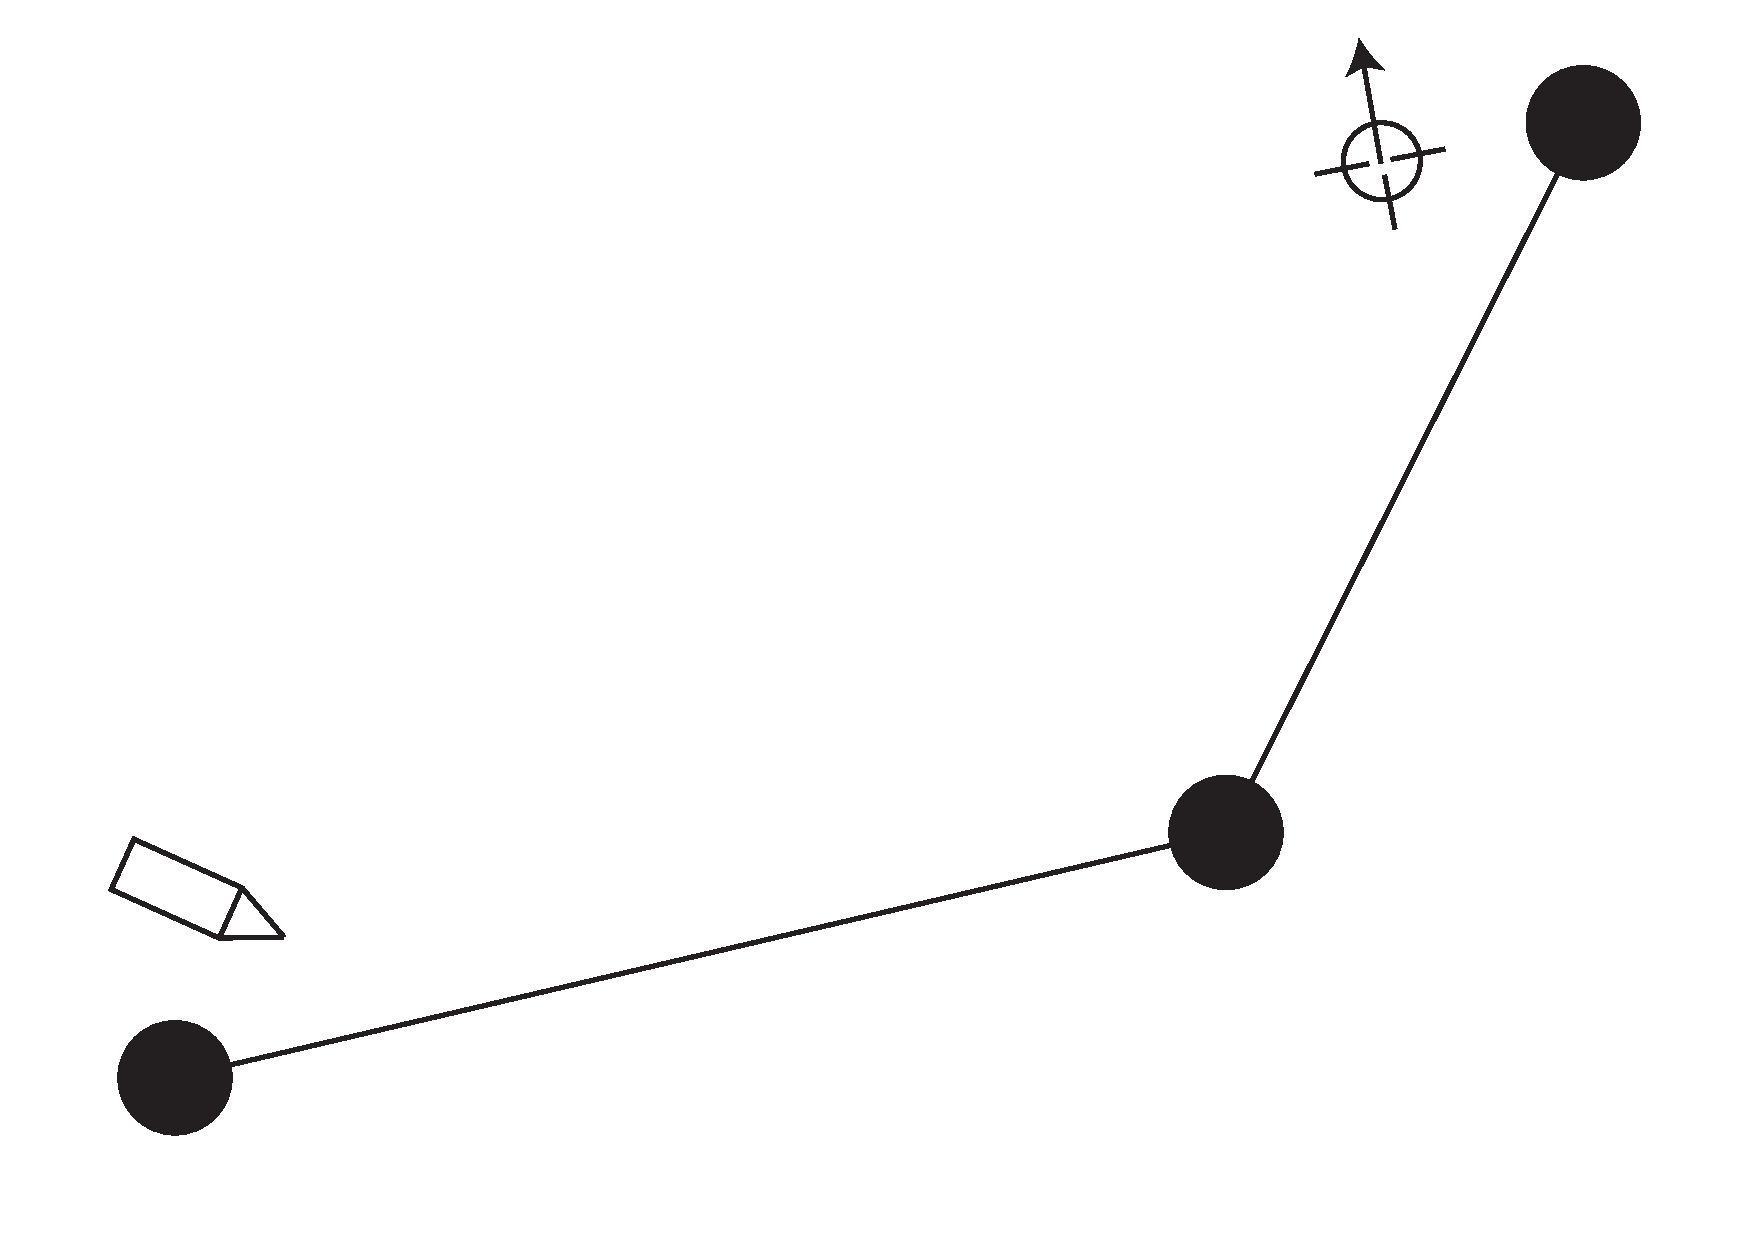
\includegraphics[width=20em]{res/pathfinding/spacelanes}
	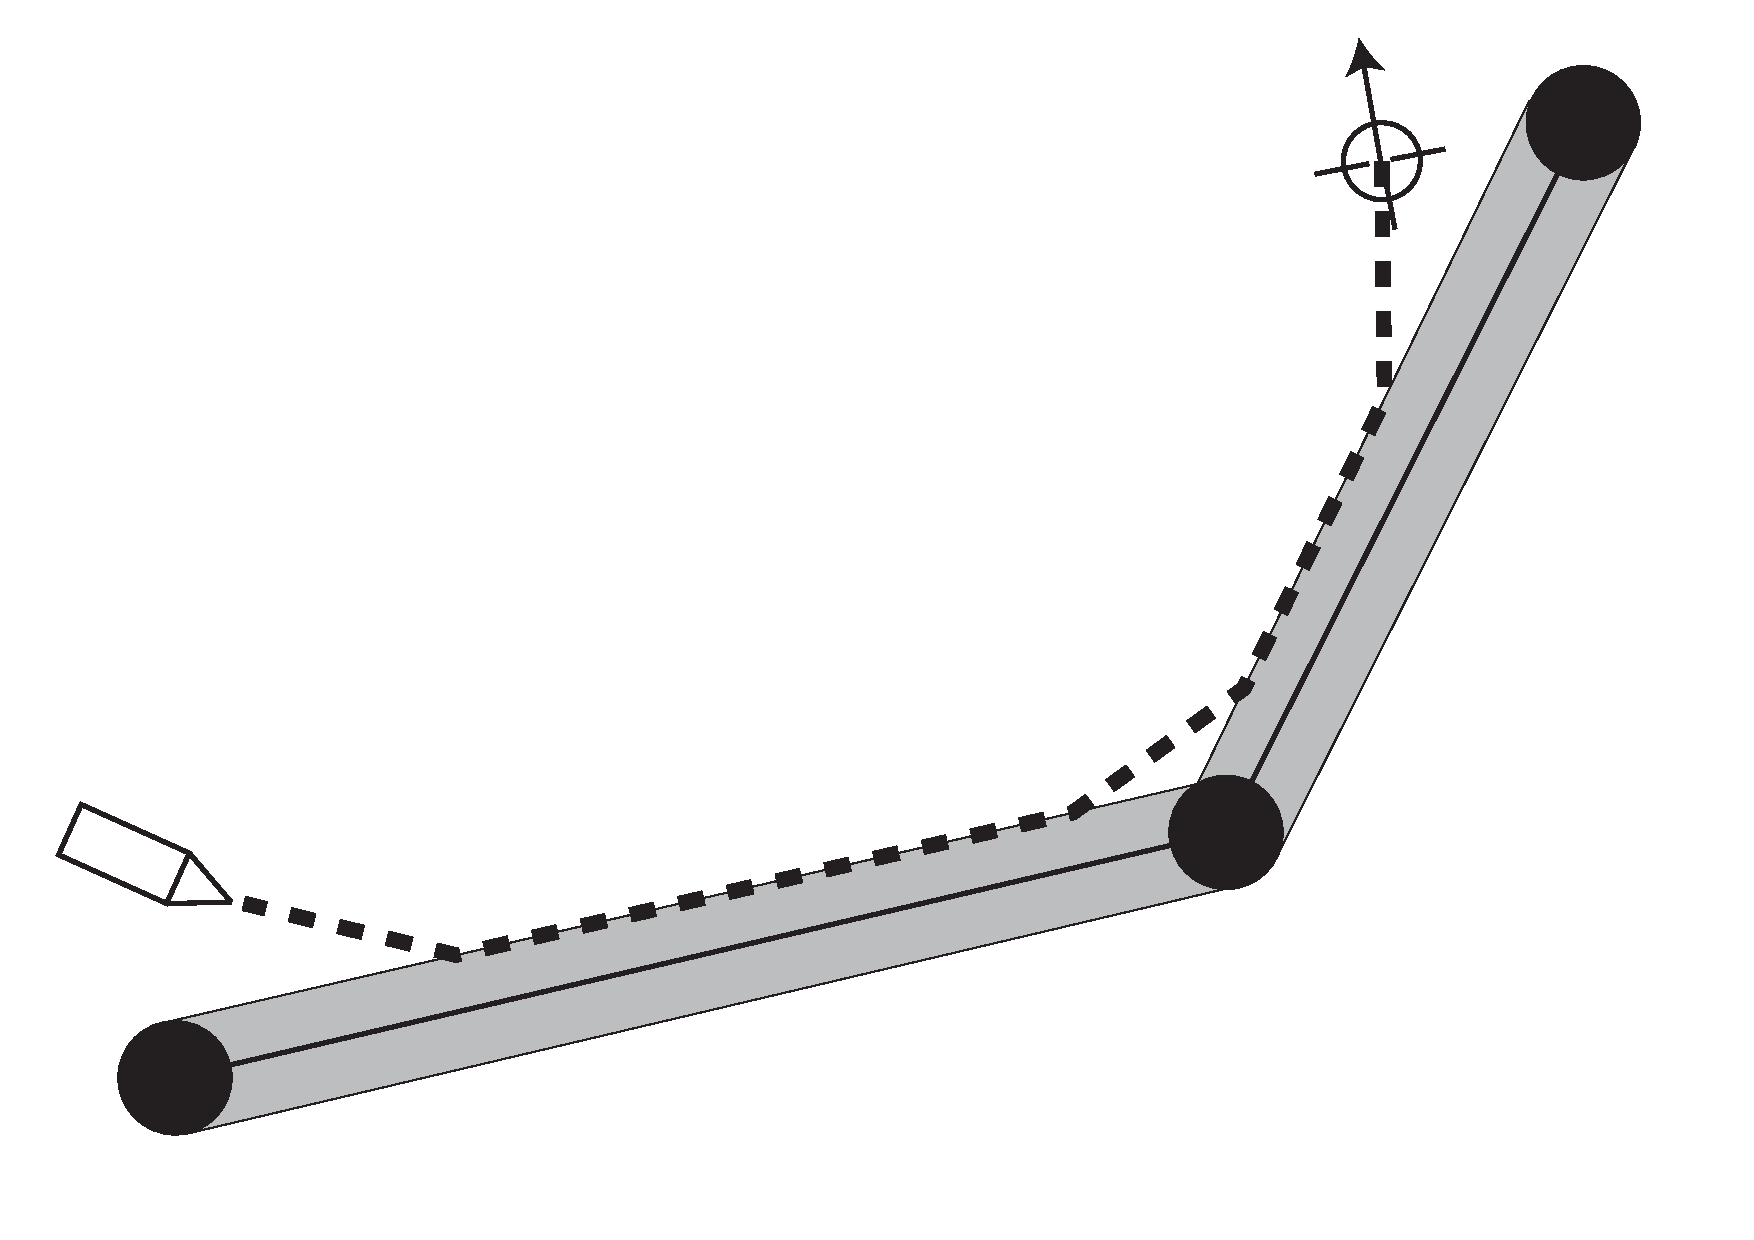
\includegraphics[width=20em]{res/pathfinding/spacelanes_ray}
	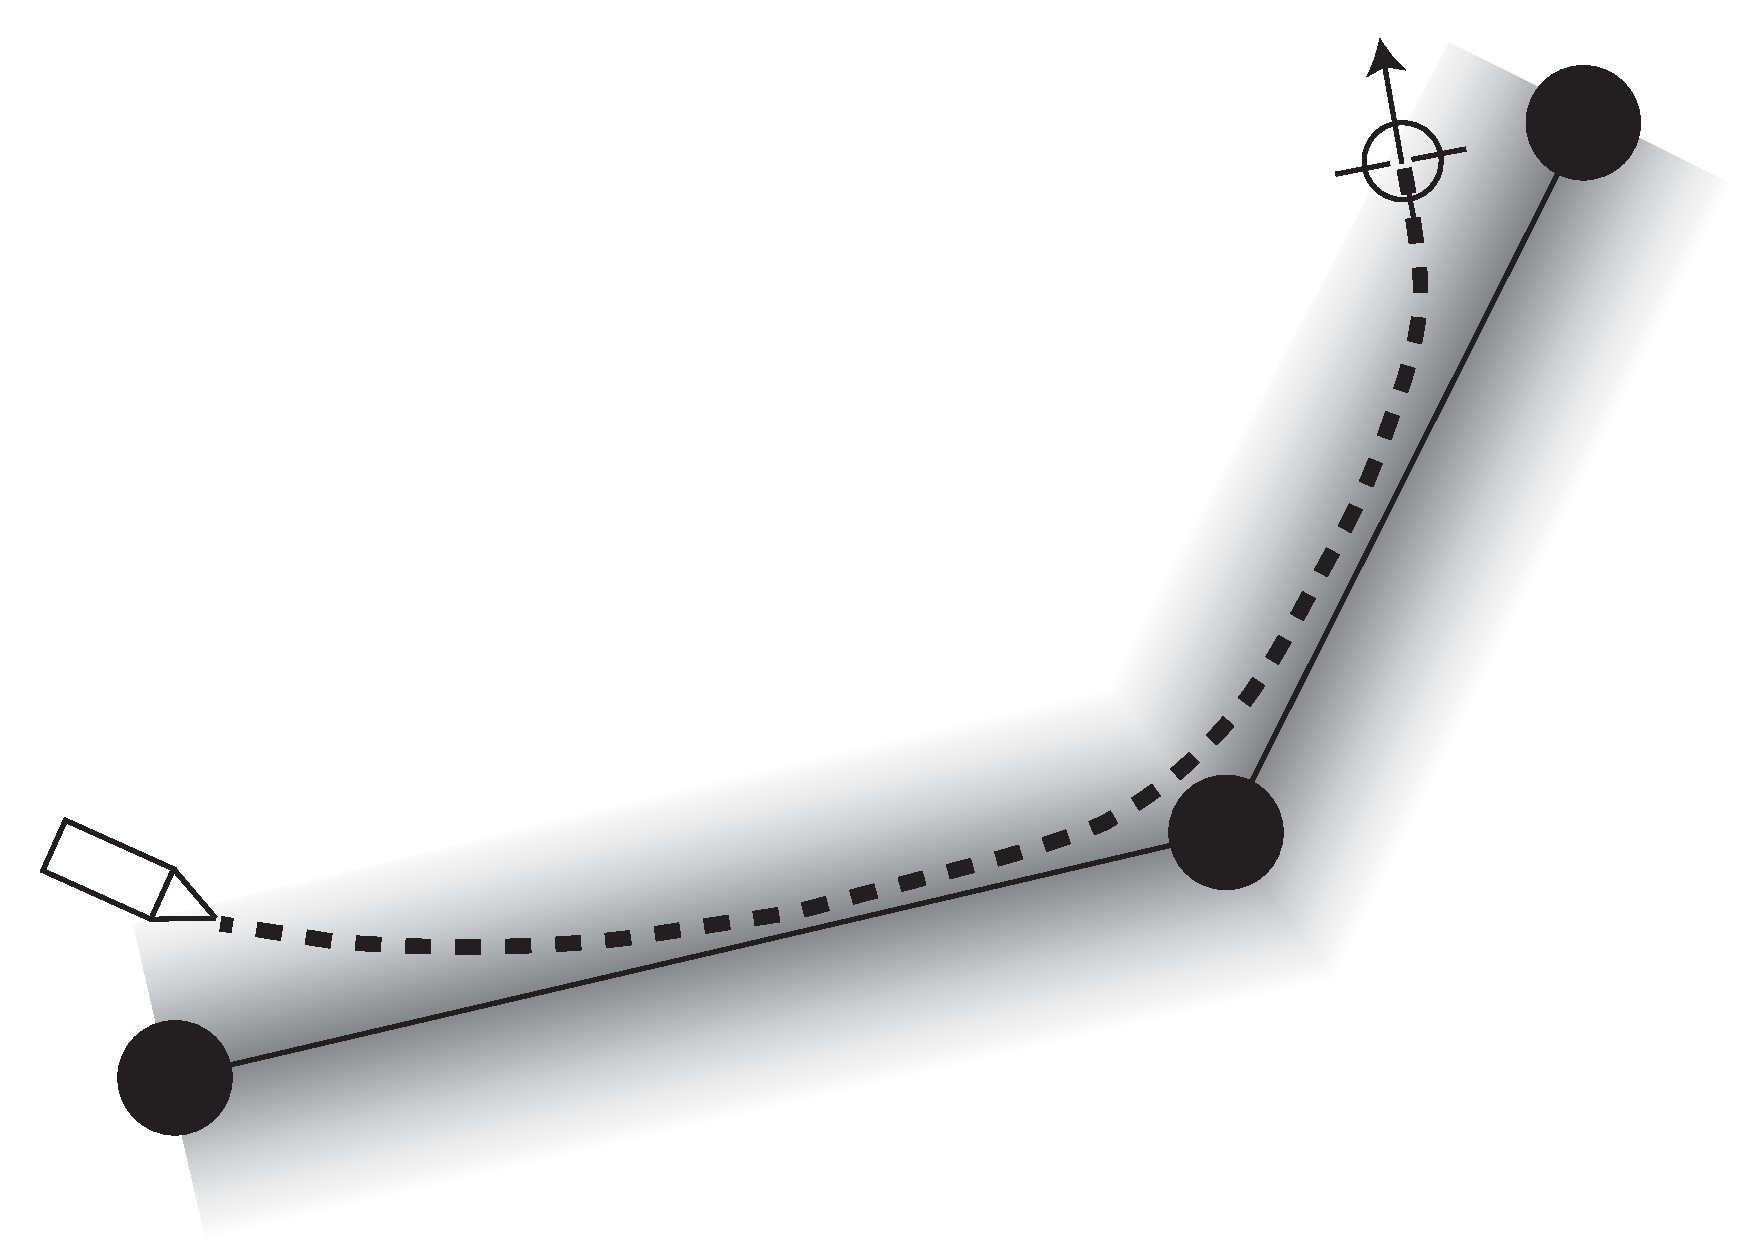
\includegraphics[width=20em]{res/pathfinding/spacelanes_field}
	\caption[Illustrations of different models for a path between current location and target utilising a space lane.]{Illustrations of different models for a path between current location and target utilising a space lane.}
	\label{fig:spacelanes}
\end{marginfigure}

Intimately related to these questions is the precise nature of the spacelane mechanics. Many different models were discussed for this during design meetings. Initial ideas on the physical mechanism of the spacelane was that they conferred an additional optional acceleration: i.e. that if a ship is proximate to a lane it could opt to undergo greater acceleration than a ship far from a lane. But as mentioned, accurately modelling acceleration in space is somewhat contrary to the gameplay aspirations of the design. 

A simpler mechanics for ships that was considered to be more suitable, is for them to have a top speed that they could reach relatively quickly; but for them to still have large turning circles. This makes their motion more similar to naval ships engaged in warfare. The interpretation of the spacelane in this model cannot be simply a gain in acceleration as this confers little benefit. Instead it is clear that the spacelane must confer an addition to top speed. A possible physical interpretation of these behaviours is that the ships are moving in some kind of ether with friction, and so will reach a terminal velocity. The spacelane is then an area with an  artificially induced lower density of ether.

Another fundamental question about the nature of the spacelane is whether its effects are immediately felt at full strength at a certain distance from it, or whether they fall off related to distance. the former is most definitely simpler, but the latter feels more natural as a mechanism. Figure~\ref{fig:spacelanes} shows the difference in the shortest paths that these approaches may generate, discounting the additional issue of ship turning.

\subsection{Algorithms for Pathfinding}
% physics hard
% bezier (not trivial)
% flow fields

\subsection{Applying A* to Sector}
% what is the problem
% why this is no trivial problem
% Why A*
Pathfinding for a game has 2 components: navigating a graph which represents the game, and the algorithm that traverses the graph to find the shortest route to a destination.
A* was chosen because it can guarantee an optimal solution, and it typically very fast if it has a good heuristic. 
Since the line of sight heuristic is applicative in this game A* will find most paths without expanding many nodes.
A* is designed to navigate discrete graphs, however In this game the sector is not a discrete graph.
The planets and space lanes on the sector can be considered a discrete graph however planets are not the only locations ships can exist at, they can move anywhere in the sector, the spaces lanes just provide a speed boost.

% conversion from sector to sector graph
A solution to this problem was to generate a discrete graph from the sector graph that could then be used by A* algorithm to find a path to destination. 
In a game such as Moon Survival on page {sec:rd:moonSurvival} the the world is already a discrete graph in the form of a 2-dimensional grid of squares, hence this can be traversed by the A* algorithm in place without having to generate a separate navigation graph.

Making a discrete navigation graph before A* could require considerable memory and CPU resources depending on the sector size.
An alternative to this solution would be to modify A* to traverse continuous graphs however designing a new algorithm to do this could cost considerable man hours to develop and will have no guarantees of finding a solution, let alone finding the optimal solution hence this alternative was dropped.

\begin{marginfigure}
	\includegraphics{res/pathfinding/PathFindingSector.pdf}
	\caption[Simple example of sector]{Simple example of sector with 3 planets: A, B, and C. Two points of interest are defined: P1 in the middle of the sector and P2 which is at planet A}
	\label{fig:pathfinding:simplesector}
\end{marginfigure}

%  - example 1
To work out how to generate a navigation graph from a sector, we needed to know the ideal path the ship would take under various circumstances before being able to implement it.
In Figure \ref{fig:pathfinding:simplesector} is an example of a sector with 3 planets.
If a ship is at P2 and wants to go to planet C, its seems rather obvious: take space lane to B then space lane to C. A space lane is faster to navigate than open space.

%  - example 2
Now consider a ship is at P1 and wants to go to planet C.
It has 3 obvious options:
\begin{itemize}
\item 
\begin{marginfigure}
	\includegraphics{res/pathfinding/PathFindingSectorOption1.pdf}
    \caption{sector navigation - option 1: path directory to planet C}
	\label{fig:pathfinding:simpleSectorOption1}
\end{marginfigure}
go directory to C across open space (Figure \ref{fig:pathfinding:simpleSectorOption1})

\item 
\begin{marginfigure}
	\includegraphics{res/pathfinding/PathFindingSectorOption2.pdf}
    \caption{sector navigation - option 2: path to B then to C}
	\label{fig:pathfinding:simpleSectorOption2}
\end{marginfigure}
goto Planet B which is close, then use its space lane to Planet C (Figure \ref{fig:pathfinding:simpleSectorOption2})

\item 
\begin{marginfigure}
	\includegraphics{res/pathfinding/PathFindingSectorOption3.pdf}
    \caption{sector navigation - option 3: path to space lane then to B then to C}
	\label{fig:pathfinding:simpleSectorOption3}
\end{marginfigure}
goto space lane between planet A and B and use it to got to B then use space lane to get to C (Figure \ref{fig:pathfinding:simpleSectorOption3}).

\end{itemize}


Traveling across open will always be considerable slow to space lanes so option 1 seems like a suboptimal choice, however did bring to light the question: How fast are space lanes?
The speed at which ships travel on space lanes needed to be defined in order to know which route is faster.

Every ship class could have 2 properties, one defining its speed in open space and one defining its speed on space lanes.
This method would allow the more specialisation amongst ships, allowing the concept of hit and run over space lanes. 
It seemed logical that a slow ship on open space should be slow on a space lane relative to a fast ship on open space, hence it seemed redundant to have 2 speed properties on a ship class.
The Method chosen was instead to define a sector property called multiplier which specifies how much faster ships are on space lanes relative to open space.
For example if the multiplayer was 3, then a ship with a speed of 10 in open space would have a speed of 30 on a space lane (3x10).
This multiplayer would be applied to all ships hence it would work on the ship's base speed defined on its ship class.
This method was simple and solved the problem.

back to the example of considering a ship at P1 which wants to go to planet C.
If we now assume a very large value for space lane multiplier, then it will greatly simplify these examples, then all space lanes will take approximately 0 seconds to use irrelevant to length, hence they are always faster over open space.
Under these conditions option 1 is slower then options 2 and 3.
Since P1 is closer to the space lane between A and B it would travel across less open space then traveling to B across open space, hence option 3 is faster then option 2.



% navigation of sector graph


% problems this method causes (not optimal solution but close)
% many nodes performance issues




\section{Assets}
<please insert shizzle here>

% ships made to look very big
% many prototypes
% merging assets with code, dynamic color
% colour selection algorithm http://gamedev.stackexchange.com/questions/46463/is-there-an-optimum-set-of-colors-for-10-players


% master copy of assets in dropbox under 4y project/laith/design
% 
\section{Configuring the Models}

% defining weapons, systems, ship classes, and fleets externally.
% information defined in yaml
% 

This section describes the method used to defines the various weapons, systems, ship classes, and fleets.
For simplicity, The weapons, systems, ship classes, and fleets will be referred to as Addons.
The reason for this name is that to add a new weapon, system, etc should be very easy from a development point of view.

Their were two options for this: defining the Addons within the code, or defining them in external resources and loading them in at runtime.
The second option is a cleaner and simpler design and allows new Addons to be defined without changing the code.

There are many data serialisation formats that are designed for this in mind, such as: XML, JSON, and YAML.
XML is highly verbose for both reading and writing, JSON requires braces for scope and quotes for any strings whereas YAML doesn't need either since it uses the white space for scoping and strings don't need quotes.
YAML is also designed to be human readable and writable, which would make manually creating and editing these Addons very easy.

It was important that new Addons should be discovered by the game when it loads, i.e. it would search for them in a given directory.
It would make the logic a little more complex but would make the interactions with the Addons very simple.
If you wanted to add an Addon simply add the a new yaml file to the correct directory, if you wanted to edit an Addon simply find the yaml file and change what values you wanted.
Unfortunately deleting Addons is not so simply, because some Addons will have dependencies on other Addons, for example a fleet may use a certain ship class, and if that ship class was deleted, that fleet would no longer be usable.
Making the deletion of Addons simple was considered, but decided against it because it would require disabling all Addons that had a dependency on a deleted Addon. This wasn't a clean design hence it is typically assumed that either no Addons are deleted or that the user knows what they are doing.
An example of a ship class defined in yaml is provided in Figure \ref{fig:configuration:corvetteYaml}


\begin{marginfigure}
	\includegraphics{res/configuration/corvetteYaml.pdf}
	\caption{
	example of ship class defined in yaml
	}
	\label{fig:configuration:corvetteYaml}
\end{marginfigure}




    
\begin{comment}

story boards:
  - client/server updates loop
  - graphics:
    - navigation
    - Paralex
  - GUI interfaces: 
    - Main Menu
    - credits
    - Game Play 
    - fleet design 
    - Results Screen
  - resources
  - planet capture
  - ship weapons arcs
  - model (sector, ship, etc):
  - AI concepts (PLAN/GOAL/ORDER)
  - path finding
    - A*
    - Bezier path
    - Flow fields
  - assets and configuration
    - assets
    - asset meta data
    - fleets
  - future work sections...
  - conclude (something)
  

\end{comment}


\begin{comment}

overall layout
--------------
game decisions
where we got to in spec
current state of game
lots of pictures

very little technical detail

lot of work on infrastructure at start



layout:
- laying the foundations:
    - got infrastructure sorted out:
        - network
        - overall glue
- alpha stage (Christmas):
    - demo stage
- leading beta stage:
    - messages/updates
    - better graphics
    - AI
- current state
- play testing and feedback
    - LIE we did lots
- future work(ryan's mum)


\end{comment}


